\chapter{Overview}
\label{cha:overview}

This chapter gives informal introduction to the RFSM language and of how to use it to describe 
FSM-based systems.

\section{Introductory example}
\label{sec:first-example}

Listing~\ref{lst:rfsm-gensig} is an example of a simple RFSM program\footnote{This program is
  provided in the distribution, under directory \texttt{examples/single/gensig}.}. This program is
used to describe and simulate the model of a calibrated pulse generator. Given an input clock
\verb|H|, with period $T_H$, it generates a pulse of duration $n \times T_H$ whenever input
\texttt{E} is set when event $H$ occurs.

\begin{lstlisting}[language=Rfsm,frame=single,numbers=left,caption=A simple RFSM
  program,label={lst:rfsm-gensig},float]
type bit = int<0:1>

fsm model gensig<n:int> (
  in h: event,
  in  e: bit,
  out s: bit)
  {
  states: E0, E1;
  vars: k: int<0..n>;
  trans: 
    E0 -- h.e=1 | k:=1; s:=1 -> E1,
    E1 -- h.k<n | k:=k+1 -> E1,
    E1 -- h.k=n | s:=0 -> E0;
  itrans: | s:=0 -> E0;
  }

input H : event = periodic (10,0,80)
input E : bit = value_changes (0:0, 25:1, 35:0)
output S : bit 

fsm g4 = gensig<4>(H,E,S)
\end{lstlisting}

The program can be divided in four parts.

\medskip
The first part (line 1) introduces a \textbf{type declaration}. The type \verb|bit| is defined as
a synonym of type \verb|int<0:1>|, \emph{i.e.} the type of integers with values between 0 and 1.

\medskip The second part (lines 3--15) gives a \textbf{generic model} of the generator behavior. The
model, named \verb|gensig|, has one parameter, \verb|n|, two inputs, \verb|h| and \verb|e|, of type
\verb|event| and \verb|bit| respectively, and one output \verb|s| of type \verb|bit|. Its behavior
is specified as a reactive FSM with two states, \verb|E0| and \verb|E1|, and one internal variable
\verb|k|. The transitions of this FSM are given after the \verb|trans:| keyword in the form :
\begin{center}
\emph{source state} \verb|--| \emph{condition} \verb'|' \emph{actions} \verb|->| \emph{destination state}
\end{center}
where \emph{condition} is the condition trigerring the transition and \emph{actions} is a list of
actions performed when then transition is enabled.  The semantics is that the transition is enabled
whenever the FSM is in the source state and the triggering condition is true. The associated actions
are then performed and the FSM moves to the destination state. For example, the first transition is
enabled whenever an event occurs on input \verb|h| and, at this instant, the value of input \verb|e|
is 1. The FSM then goes from state \verb|E0| to state \verb|E1| and sets its internal variable 
\verb|k| and its output \verb|s| to 1. The \emph{initial transition} of the FSM is given 
after the \verb|itrans:| keyword in the form :
\begin{center}
\verb'|' \emph{initial actions} \verb|->| \emph{initial state}
\end{center}
Here the FSM is initially in state \verb|E0| with output \verb|s| set to 0.

A graphical representation of the \verb|gensig| model is given in
Fig.~\ref{fig:rfsm-gensig-model} (this representation was actually automatically generated from the
program in Listing~\ref{lst:rfsm-gensig}, as explained in Chap.~\ref{cha:rfsmc}). 

\begin{figure}[h]
   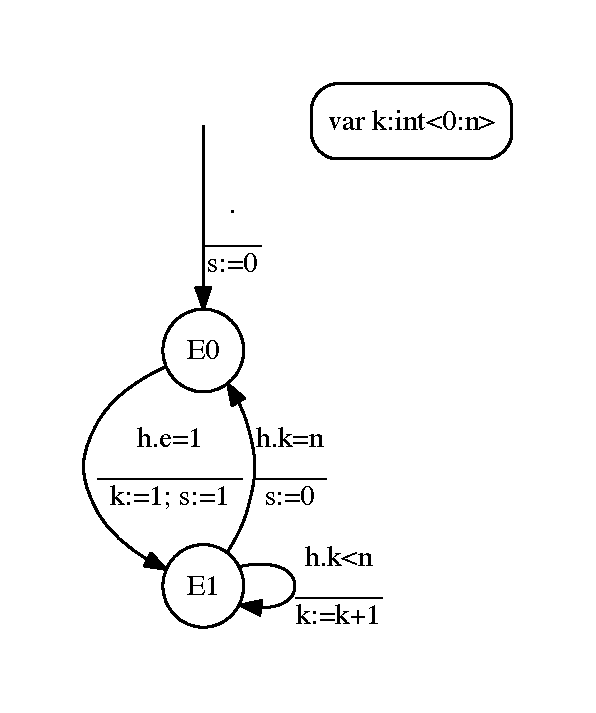
\includegraphics[height=8cm]{figs/gensig-model}
   \centering
  \caption{A graphical representation of FSM model defined in Listing~\ref{lst:rfsm-gensig}}
  \label{fig:rfsm-gensig-model}
\end{figure}

Note that, at this level, the value of the parameter \verb|n|, used in the type of the internal variable
\verb|k| (line 9) and in the transition conditions (lines 12 and 13) is left unspecified, making the
\verb|gensig| model a \emph{generic} one.

\medskip The third part of the program (lines 17--19) lists \textbf{global inputs and
  outputs}\footnote{In case of multi-FSM programs, this part will also contains the declaration of
  \emph{shared} events and variables. See Sec.~\ref{sec:globals}.}.  For global outputs the
declaration simply gives a name and a type.  For global inputs, the declaration also specifies the
\textbf{stimuli} which are attached to the corresponding input for simulating the system. The
program of Listing~\ref{lst:rfsm-gensig} uses two kinds of stimuli\footnote{See
  Sec.~\ref{sec:globals} for a complete description of stimuli.}. The stimuli attached to input
\verb|H| are declared as \emph{periodic}, with a period of 10 time units, a start time of 0 and a
end time of 80. This means than an event will be produced on this input at time 0, 10, 20, 30, 40,
50, 60, 70 and 80. The stimuli attached to input \verb|E| say that this input will respectively take
value 0, 1 and 0 at time 0, 25 and 35 (thus producing a ``pulse'' of duration 10 time units starting
at time 25).

\medskip
The last part of the program (line 21) consists in building the global model of the system by
\emph{instanciating} the FSM models.
Instanciating a model creates a ``copy'' of this model for which
\begin{itemize}
\item the generic parameters (\verb|n| here) are now bound to actual values (4 here),
\item the inputs and outputs are connected to the global inputs or outputs. 
\end{itemize}

\medskip
A graphical representation of the system described in Listing~\ref{lst:rfsm-gensig} is given in
Fig.~\ref{fig:rfsm-gensig-top}\footnote{Again, this representation was actually automatically generated from the
program in Listing~\ref{lst:rfsm-gensig}, as explained in Chap.~\ref{cha:rfsmc}}. 

\begin{figure}[h]
   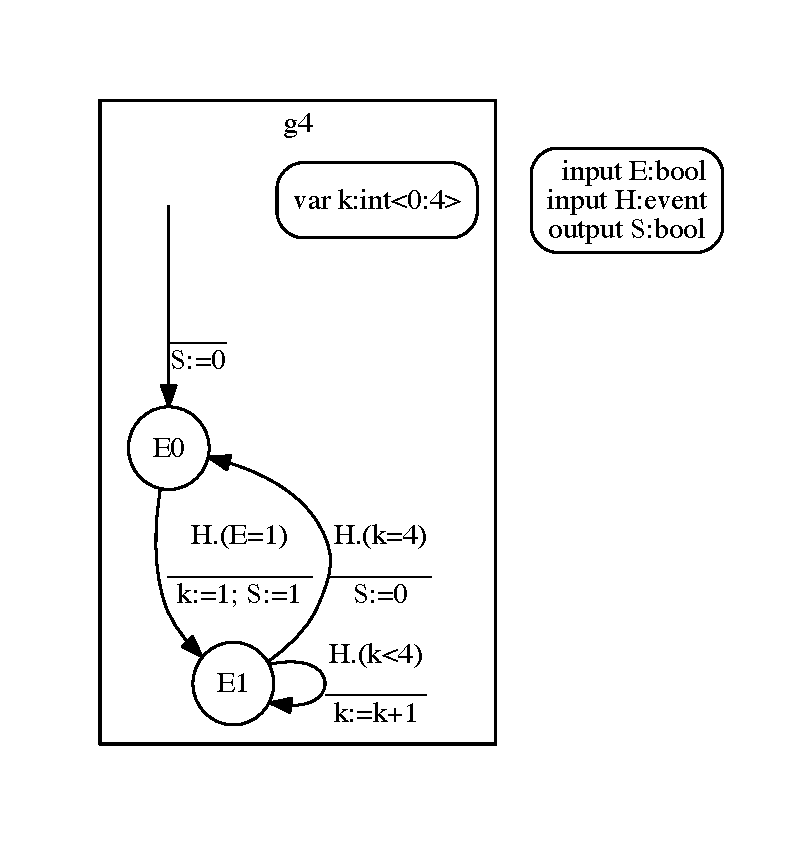
\includegraphics[height=8cm]{figs/gensig-top}
   \centering
  \caption{A graphical representation of system described in Listing~\ref{lst:rfsm-gensig}}
  \label{fig:rfsm-gensig-top}
\end{figure}

\subsection*{Simulating}
\label{sec:simulating-1}

Simulating the program means computing the reaction of the system to the input stimuli. Simulation
can be performed the RFSM command-line compiler or the IDE (see Chap.~\ref{cha:rfsmc} and
\ref{cha:gui} resp.). It produces a set of
\emph{traces} in VCD (Value Change Dump) format which can visualized using \emph{waveform viewers}
such as \texttt{gtkwave}. The simulation results for the program in Listing~\ref{lst:rfsm-gensig}
are illustrated in Fig.~\ref{fig:rfsm-gensig-chrono}.

\begin{figure}[h]
   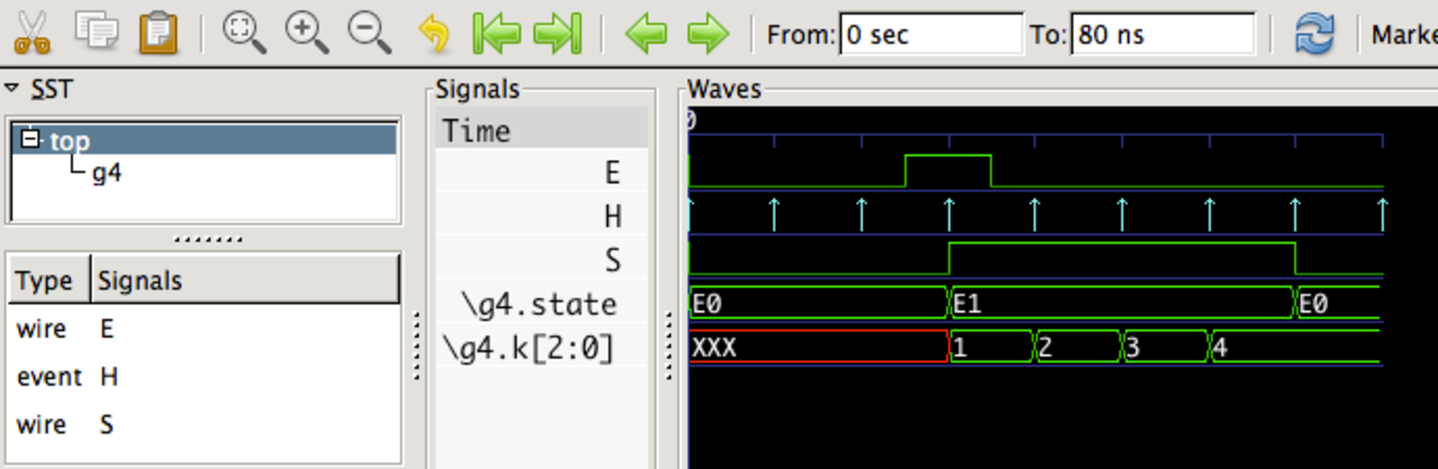
\includegraphics[width=\textwidth]{figs/gensig-chrono}
   \centering
  \caption{Simulation results for the program in Listing~\ref{lst:rfsm-gensig}, viewed using
    \texttt{gtkwave}}
  \label{fig:rfsm-gensig-chrono}
\end{figure}

\subsection*{Code generation}
\label{sec:code-generation-1}

RFSM can also generate code implementing the described systems simulation and/or
integration to existing applications.

\medskip
Currently, three backends are provided :
\begin{itemize}
\item a backend generating a C-based implementation of each FSM instance,
\item a backend generating a \emph{testbench} implementation in SystemC (FSM instances + stimuli
  generators),
\item a backend generating a \emph{testbench} implementation in VHDL (FSM instances + stimuli
  generators).
\end{itemize}

\medskip
The target language for the C backend is a C-like language augmented with
\begin{itemize}
\item a \verb|task| keyword for naming generated behaviors,
\item \verb|in|, \verb|out| and \verb|iinout| keywords for identifying inputs and outputs,
\item a builtin \verb|event| type,
\item primitives for handling events : \verb|wait_ev()|, \verb|wait_evs()| and
  \verb|notify_ev()|. 
\end{itemize}
The idea is that the generated code can be turned into an application for a multi-tasking operating
system by providing actual implementations of the corresponding constructs and primitives.

\medskip
For the SystemC and VHDL backends, the generated code can actually be compiled and executed for
simulation purpose and. The FSM implementations generated by the VHDL backend can also be
synthetized to be implemented hardware using hardware-specific tools\footnote{We use the
  \textsc{quartus} toolchain from Intel/Altera.}. 

\medskip
Appendices C1, C2 and C3 respectively give the C and SystemC code generated from the example in
Listing~\ref{lst:rfsm-gensig}. 

\section{The RFSM language}
\label{sec:rfsm-language}

This section is more thorough presentation of the RFSM language introduced in the previous
section. This presentation is deliberately informal. The complete language syntax can
be found in Appendix~A.

\subsection{Types}
\label{sec:types}

There are two categories of types~: builtin types and user defined types.

\medskip
\textbf{Builtin types} are : \texttt{bool}, \texttt{int}, \texttt{float} and \texttt{event}.

\step Objects of type \texttt{bool} can have only two values : \texttt{true} and \texttt{false}.

\step The type \texttt{int} can be refined using a \emph{range annotation}. The type
\verb|int<lo:hi>| designates integer values ranging from \verb|lo| to \verb|hi|. The range limits
\verb|lo| and \verb|hi| can be constants or expressions whose value can be computed as compile
time (expressions involving parameter values, as exemplified line 9 in
Listing~\ref{lst:rfsm-gensig}).  

\step The operations on values of type \texttt{int} are : \verb|+|, \verb|-|, \verb|*|, \verb|/| and
\verb|%| (modulo).

\step The operations on values of type \texttt{float} are : \verb|+.|, \verb|-.|, \verb|*.|,
\verb|/.| (the dot suffix is required to distinguish them from the corresponding operations on
\texttt{int}s).

\medskip
\textbf{User defined types} are either \emph{type abbreviations} or \emph{enumerations}.

\step Type abbreviations are introduced with the following declaration
\begin{center}
  \framebox{\lstinline[language=Rfsm]{type typename = type_expression}}
\end{center}
Each occurrence of the defined type in the program is actually substituted by the corresponding type
expression. Type expressions in type abbreviations are currently limited to builtin types.
An example of type abbreviation has been given in the program of Listing~\ref{lst:rfsm-gensig}. 

\medskip
\textbf{Enumerated types}  are introduced with the following declaration
\begin{center}
  \framebox{\lstinline[language=Rfsm]|type typename = \{ C1, ..., Cn \}|}
\end{center}
where \verb|C1|, \ldots, \verb|Cn| are the enumerated values, each being denoted by an identifier
starting with an uppercase letter. For example : 
\begin{center}
  \example{\lstinline[language=Rfsm]|type color = \{ Red, Green, Orange \}|}
\end{center}


\subsection{FSM models}
\label{sec:fsm-models}

An FSM model, introduced by the \verb|fsm model| keywords, describes the interface and behavior of a
\emph{reactive finite state machine}. A reactive finite state machine is a finite state machine
whose transitions can only be caused by the occurrence of \emph{events}.

\begin{center}
\framebox{\lstinline[language=Rfsm]|fsm model <interface> { <body> }|}
\end{center}

\medskip
The \textbf{interface} of the model gives its name, a list of parameters (which can be empty) and a
list of inputs and outputs. All parameters and IOs are typed. Inputs and outputs are explicitely
tagged. An IO tagged \verb|inout| acts both as input and output (it can be read and written by the
model). Inputs and outputs are listed between \verb|(...)|. Parameters, if present are given between
\verb|<...>|. Examples :

\begin{center}
\example{\lstinline[language=Rfsm]|fsm model cntmod8 (in h: event, out s: int<0..7>) \{ ... \}|}
\end{center}

\begin{center}
\example{\lstinline[language=Rfsm]|fsm model gensig<n:int> (in h: event, in  e: bit, out s: bit) \{ ... \}|}
\end{center}

\begin{center}
\example{\lstinline[language=Rfsm]|fsm model update (in top: event, inout  lock: bool) \{ ... \}|}
\end{center}

\medskip
The model \textbf{body}, written between \verb|{...}|, generally comprises four sections :
\begin{itemize}
\item a section giving the list of \emph{states},
\item a section introducing local (internal) \emph{variables},
\item a section giving the list of \emph{transition},
\item a section specifying the \emph{initial transition}.
\end{itemize}

Each section starts with the corresponding keyword (\verb|states:|, \verb|vars:|, \verb|trans:| and
\verb|itrans:| resp.) and ends with a semi-colon.

\begin{center}
\framebox{\lstinline[language=Rfsm]| fsm model ... ( ... ) \{ states: ...; vars: ...; trans: ...; itrans: ...; \}|}
\end{center}

\subsubsection*{States}
\label{sec:states}


The \verb|states:| section gives the set of internal states, as a comma-separated list of
identifiers (each starting with a uppercase letter). Example :

\begin{center}
\example{\lstinline[language=Rfsm]|states: Idle, Wait1, Wait2, Done;|}
\end{center}

\subsubsection*{Variables}
\label{sec:variables}

The \verb|vars:| section gives the set of internal variables, each with its type. Example :

\begin{center}
\example{\lstinline[language=Rfsm]|vars: cnt: int, stop: bool;|}
\end{center}

The type of a variable may depend on parameters listed in the model interface. Example

\begin{center}
\example{\lstinline[language=Rfsm]|fsm gensig<n: int> (...) \{ ... vars: k: int<0..n>; ... \}|}
\end{center}

The \verb|vars:| section may be omitted.

\subsubsection*{Transitions}
\label{sec:transitions}

The \verb|trans:| section gives the set of transitions between states. Each transition is denoted

\begin{center}
\framebox{\lstinline[language=Rfsm]{src_state -- condition | actions -> dst_state}}
\end{center}

where
\begin{itemize}
\item \emph{src\_state} and \emph{dst\_state} respectively designates the source state and destination state,
\item \emph{condition} is the condition trigerring the transition,
\item \emph{actions} is a list of actions performed when then transition is enabled.
\end{itemize}

\medskip The semantics is that the transition is enabled whenever the FSM is in the source state and
the triggering condition is true. The associated actions are then performed and the FSM moves to the
destination state.

\medskip
A \textbf{condition} must involve exactly one \emph{triggering event} and, possibly, a conjunction of boolean
conditions called \emph{guards}. The triggering event must be listed in the inputs. The guards may
involve inputs and/or internal variables.

\medskip The \textbf{actions} associated to a transition consists in modifications of the outputs
and/or internal variables or emissions of events. Modifications of outputs and internal variables
are denoted

\begin{center}
\framebox{\lstinline[language=Rfsm]{id := expr}}
\end{center}

where \emph{id} is the name of the output (resp. variable) and \emph{expr} an expression involving
inputs, outputs and variables and operations allowed on the corresponding types. The set of allowed
operations is given in Table~\ref{tab:type-ops}.

\begin{table}
\begin{minipage}[c]{1.0\linewidth}
\small
\begin{center}
\begin{tabular}{|l|l|} \hline
{\tt int}       & {\tt + - * / mod = != > < >= <=} \\  \hline
{\tt bool}      & {\tt = !=} \\ \hline 
{\tt enumeration}     & {\tt = !=} \\  \hline
\end{tabular}
\caption{Operations on types}
\label{tab:type-ops}
\end{center}
\end{minipage}
\end{table}

\medskip
The action of emitting of an event  is simply denoted by the name of this event.

\medskip
Examples :

\begin{center}
\example{\lstinline[language=Rfsm]'S0 -- top -> S1'}
\end{center}

In the above example, the enclosing FSM switches from state \verb|S0| to state \verb|S1| when the
event \verb|top| occurs. 

\begin{center}
\example{\lstinline[language=Rfsm]'Idle -- Clic | ctr:=0; Received -> Wait'}
\end{center}

In the above example, the enclosing FSM switches from state \verb|Idle| to state \verb|Wait|, resetting the internal variable
  \verb|ctr| to 0 and emitting event \verb|Received| whenever an event occurs on its \verb|Clic| input.

\begin{center}
\example{\lstinline[language=Rfsm]'Wait -- Top.ctr<8 | ctr:=ctr+1 -> Wait'}
\end{center}

In the above example, the enclosing FSM stays in state \verb|Wait| but increments the internal
variable \verb|ctr| whenever an event \verb|Top| occurs and that, \emph{at this instant}, the
value of variable \verb|ctr| is smaller than 8. 

\medskip
Expressions may also involve the C-like ternary conditional operator \verb|?:|.
For example, in the example below, the enclosing FSM stays in state \verb|S0| but updates the variable \verb|k|
at each occurrence of event \verb|H| so that is incremented if its current value is less than 8 or
reset to 0 otherwise.

\begin{center}
\example{\lstinline[language=Rfsm]'S0 -- H | k:=k<8?k+1:0 -> S0'}
\end{center}


\medskip
The set of actions may be empty. In this case, the transition is denoted :

\begin{center}
\framebox{\lstinline[language=Rfsm]{src_state -- condition -> dst_state}}
\end{center}

\subsubsection*{Initial transition}
\label{sec:initial-transition}

The \verb|itrans:| section specifies the initial transition of the FSM. This transition is denoted~:

\begin{center}
\framebox{\lstinline[language=Rfsm]{| actions -> init_state}}
\end{center}

where \emph{init\_state} is the initial state and \emph{actions} a list of actions to be performed
when initializing the FSM. The latter can be empty. in this case the initial transition is simply
denoted~:

\begin{center}
\framebox{\lstinline[language=Rfsm]{-> init_state}}
\end{center}

\subsection{Globals}
\label{sec:globals}

Globals are used to connect model instances to the external world or to other instances.

\subsubsection*{Inputs and outputs}
\label{sec:inputs-outputs}

Interface to the external world are represented by \verb|input| and \verb|output| objects.

\step For outputs the declaration simply gives a name and a type~:

\begin{center}
\framebox{\lstinline[language=Rfsm]'output name : typ'}
\end{center}

\step For inputs, the declaration also specifies the \textbf{stimuli} which are attached to the
corresponding input for simulating the system.
\begin{center}
\framebox{\lstinline[language=Rfsm]'input name : typ = stimuli'}
\end{center}

There are three types of stimuli~:
periodic and
sporadic stimuli for inputs of type \verb|event| and value changes for scalar inputs.

\medskip
Periodic stimuli are specified with a period, a starting time and an ending time.

\begin{center}
\framebox{\lstinline[language=Rfsm]'periodic(period,t0,t1)'}
\end{center}

Sporadic stimuli
are simply a list of dates at which the corresponding input event occurs.

\begin{center}
\framebox{\lstinline[language=Rfsm]'sporadic(t1,...,tn)'}
\end{center}

Value changes are given as
list of pairs \verb|t:v|, where \verb|t| is a date and \verb|v| the value assigned to the
corresponding input at this date. 

\begin{center}
\framebox{\lstinline[language=Rfsm]'value_changes(t1:v1,...,tn:vn)'}
\end{center}

\medskip
Examples:

\begin{center}
\example{\lstinline[language=Rfsm]'input Clk: event = periodic(10,10,120)'}
\end{center}

The previous declaration declares \verb|Clk| as a global input producing periodic events with period 10, starting
  at t=10 and ending at t=100\footnote{Note that, at this level, there's no need for an absolute
    unit for time.}.

\begin{center}
\example{\lstinline[language=Rfsm]'input Clic: event = sporadic(25,75,95)'}
\end{center}

The previous declaration declares \verb|Clic| as a global input producing events at t=25, t=75 and
  t=95.

\begin{center}
\example{\lstinline[language=Rfsm]'input E : bool = value_changes (0:false, 25:true, 35:false)'}
\end{center}

The previous declaration declares \verb|E| as a global boolean input taking value \texttt{false} at
t=0, \texttt{true} at t=25 and \texttt{false} again at t=35.

\subsubsection*{Shared objects}
\label{sec:shared}

Shared objects are used to represent interconnexions between FSM instances. This situation only
occurs when the system model involves several FSM instances and when the input of a given instance
is provided by the output of another one (see Section~\ref{sec:fsm-instances}).

\step For shared objects the declaration simply gives a name and a type~:

\begin{center}
\framebox{\lstinline[language=Rfsm]'shared name : typ'}
\end{center}

\subsection{Instances and system}
\label{sec:fsm-instances}

The last section of an RFSM program constructs the description of the system by instanciating
-- and, possibly, inter-connecting -- the previously FSM models.

\medskip
Instanciating a model creates a ``copy'' of the corresponding FSM for which
\begin{itemize}
\item the parameters of the model are bound to their actual value,
\item the declared inputs and outputs are connected to global inputs, outputs or shared
  objects.
\end{itemize}

\medskip
The syntax for declaring a model instance is as follows~:

\begin{center}
\framebox{\lstinline[language=Rfsm]'fsm inst_name = model_name<param_values>(actual_ios)'} 
\end{center}

where
\begin{itemize}
\item \emph{inst\_name} is the name of the created instance,
\item \emph{model\_name} is the name of the instanciated model,
\item \emph{param\_values} is a comma-separated list of values to be assigned to the formal
  (generic) parameters,
\item \emph{actual\_ios} is a comma-separated list of global inputs, outputs or shared objects to be
  connected to the instanciated model.
\end{itemize}

Binding of parameter values and IOs is done by position. Of course the number and respective types
of the formal and actual parameters (resp. IOs) must match.

\medskip
For example, the last line of the program given in Listing~\ref{lst:rfsm-gensig}

\begin{center}
\example{\lstinline[language=Rfsm]'fsm g4 = gensig<4>(H,E,S)'}
\end{center}

creates an instance of model \verb|gensig| for which \verb|n=4| and whose inputs (resp. output) are
connected to the global inputs (resp. output) \texttt{H} and \texttt{E} (resp. \texttt{S}).

\subsubsection*{Multi-FSM models}
\label{sec:multi-fsm-models}

It is of course possible to build a system model as a \emph{composition} of FSM instances.  An
example is given in Listing~\ref{lst:rfsm-cntmod8}. The system is a simple modulo 8 counter, here
described as a combination of three event-synchronized modulo 2 counters\footnote{This program is
  provided in the distribution, under directory \texttt{examples/multi/ctrmod8}.}.

\medskip
Here a single FSM model (\texttt{cntmod2}) is instanciated thrice, as \texttt{C0}, \texttt{C1} and
\texttt{C2}. These instances are synchronized using two \textbf{shared events}, \texttt{R0} and \texttt{R1}. 

\medskip
The graphical representation of the program is given in Fig.~\ref{fig:rfsm-cntmod8-top}. Simulation
results are illustrated in Fig~\ref{fig:rfsm-cntmod8-vcd}. 

\begin{lstlisting}[language=Rfsm,frame=single,numbers=left,caption=A multi-model RFSM
  program,label={lst:rfsm-cntmod8},float]
fsm model cntmod2 (
  in h: event,
  out s: int<0:1>,
  out r: event)
  {
  states: E0, E1;
  trans:
    E0 -- h | s:=1 -> E1,
    E1 -- h | r; s:=0 -> E0;
  itrans: | s:=0 -> E0;
  }

input H: event = periodic(10,10,100)
output S0: int<0:1>
output S1: int<0:1>
output S2: int<0:1>
output R2: event

shared R0: event
shared R1: event

fsm C0 = cntmod2(H,S0,R0) 
fsm C1 = cntmod2(R0,S1,R1) 
fsm C2 = cntmod2(R1,S2,R2) 
\end{lstlisting}

\begin{figure}[h]
   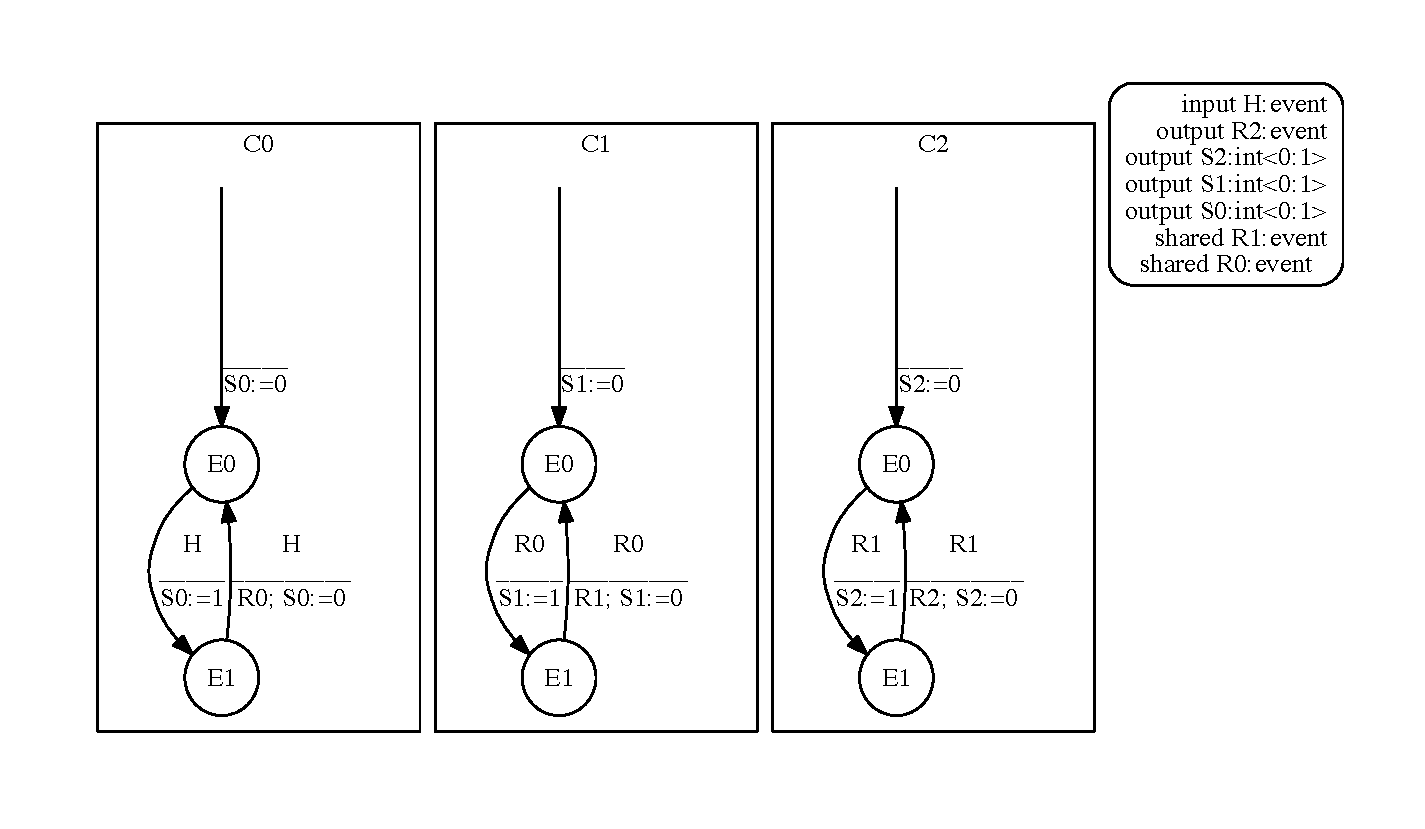
\includegraphics[height=9cm]{figs/ctrmod8-top}
   \centering
  \caption{A graphical representation of program described in Listing~\ref{lst:rfsm-cntmod8}}
  \label{fig:rfsm-cntmod8-top}
\end{figure}

\begin{figure}[h]
   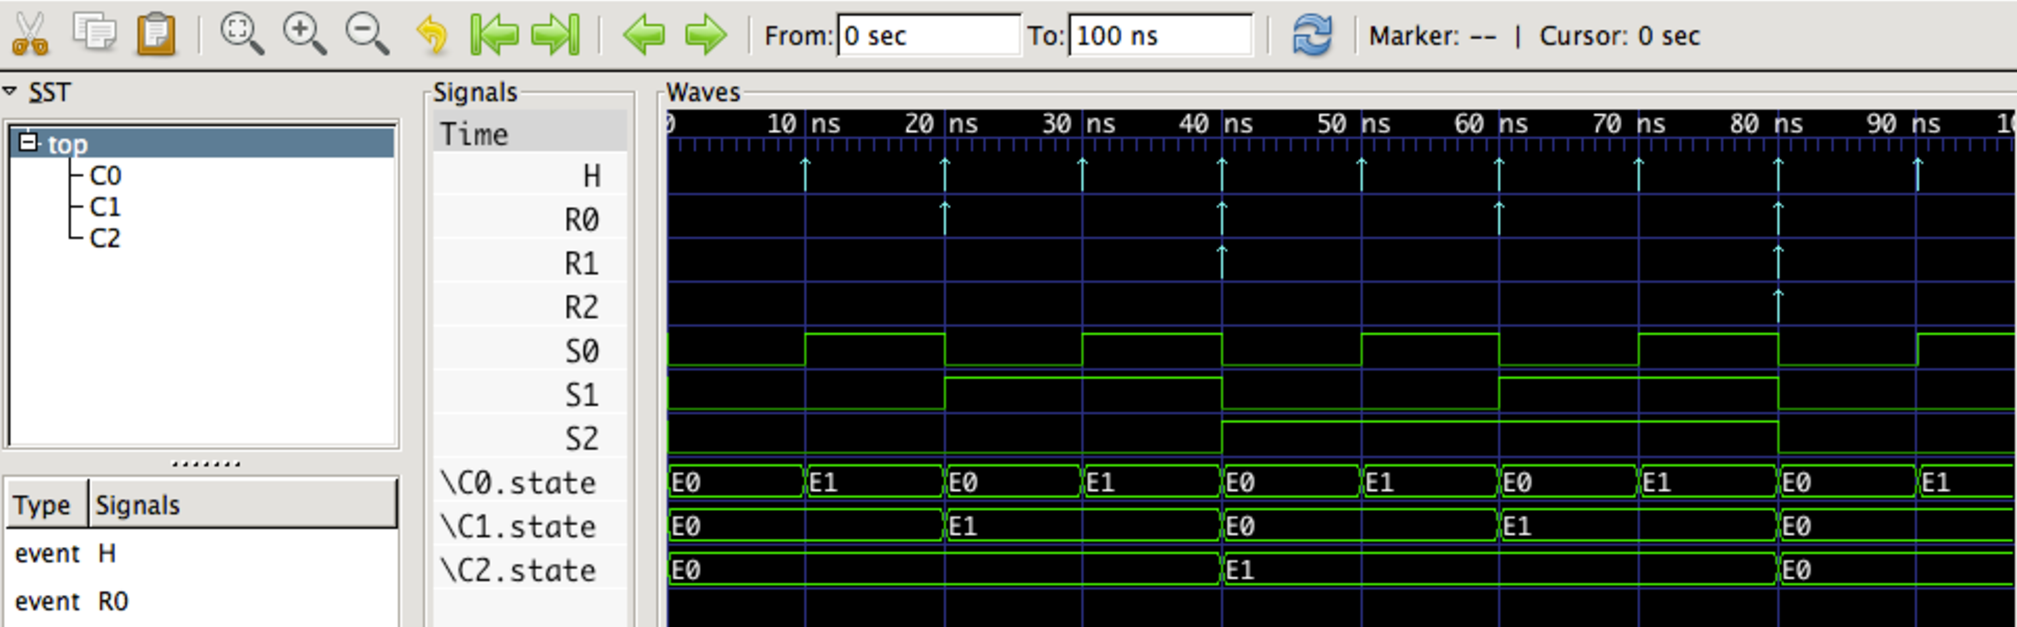
\includegraphics[width=\textwidth]{figs/ctrmod8-chrono}
   \centering
  \caption{Simulation results for the program in Listing~\ref{lst:rfsm-cntmod8}}
  \label{fig:rfsm-cntmod8-vcd}
\end{figure}

\subsection{Semantic issues}
\label{sec:semantic-issues}

This presentation of the language has deliberately focused on syntax. Formalizing the semantics of programs made of
reactive finite state machines -- and in particular when several of these machines are interacting
-- is actually far from trivial and will not be carried out here. 

Instead, this section will describe some ``practical'' problems that may arise when simulating such
systems and how the language currently addresses them, without delving too much into the underlying
semantics issues\footnote{This is not that these issues do not deserve a formal treatment. Of
  course, they do ! But we think we this document is not the right place to do it.}.

\subsubsection{Priorities}
\label{sec:priorities}

The FSM models involved in programs should normally be \emph{deterministic}. In other words, a
situation where several transitions are enabled at the same instant should normally never arise. But
this condition may actually be difficult to enforce, especially for models reacting to several input
events. Consider for example, the model described in Listing~\ref{lst:rfsm-prio-pb}. This model
describes a (simplified) stopwatch. It starts counting seconds (materialized by event \verb|sec|)
as soon as event \verb|startstop| occurs and stops as soon as it occurs again.

\begin{lstlisting}[language=Rfsm,frame=single,numbers=left,caption=A program showing a potentially non-deterministic
  model,label={lst:rfsm-prio-pb},float]
fsm model chrono (
     in sec: event,
     in startstop: event,
    out aff: int)
  {
  states: Stopped, Running;
  vars: ctr: int;
  trans:
    Stopped -- startstop | ctr:=0; aff:=0 -> Running,
    Running -- sec | ctr:=ctr+1; aff:=ctr -> Running,
    Running -- startstop -> Stopped;
  itrans: -> Stopped;
  }

input StartStop: event = sporadic(25,70)
input H:event = periodic(10,10,110)
output Aff: int

fsm c1 = chrono(H,StartStop,Aff)
\end{lstlisting}

The problem is that if both events occur simultaneously  then
both the transitions at line 10 and 11 are enabled. In fact, here's the error message produced by
the compiler when trying to simulate the above program :

\small
\begin{verbatim}
Error when simulating FSM c1: non deterministic transitions found at t=70:
	- Running--h|ctr:=ctr+1; aff:=ctr->Running[0]
	- Running--startstop->Stopped[0]
\end{verbatim}
\normalsize

Of course, this could be avoided by modifying the stimuli attached to input \verb|StartStop| so that the
corresponding events are never emitted at time $t=n\times 10$. But this is, in a sence, cheating,
since this event is supposed to modelize user interaction which occur, by essence, at impredictible
dates. 

The above problem can be solved by assigning a \emph{priority} to transitions. In the current
implementation, this is achieved by tagging some transitions as ``high priority''
transitions\footnote{Future versions may evolve towards a more sophisticated mechanism allowing
  numeric priorities.}.  When several transitions are enabled, if one is tagged as ``high priority''
than it is automatically selected\footnote{If none (resp. several) is (resp. are) tagged, the
  conflict remains, of course.}. 

Syntaxically, tagging a transition is simply achieved by prefixing it with a ``\verb|*|''. In the
case of the example above, the modified program is given in
Listing~\ref{lst:rfsm-prio-solved}. Tagging the last transition is here equivalent to give to the
\verb|startstop| precedence against the \verb|h| event when the model is in state
\verb|Running|.

\begin{lstlisting}[language=Rfsm,frame=single,numbers=left,caption=A rewriting of the model defined
  in Listing~\ref{lst:rfsm-prio-pb}, label={lst:rfsm-prio-solved},float]
fsm model chrono (...)
  {
  ...
  trans:
    ...
    Running -- sec | ctr:=ctr+1; aff:=ctr -> Running,
    *Running -- startstop -> Stopped;
  itrans: -> Stopped;
  }
...
\end{lstlisting}

\subsubsection{Sequential vs. synchronous actions}
\label{sec:sequ-vs.-synchr}

An important question is whether, when a transition specifying \emph{several actions} to be
performed is taken, the corresponding actions are performed sequentially or not. 

Consider for example, the following transition, in which \verb|x| and \verb|y| are internal
variables of the enclosing FSM :

\begin{center}
\example{\lstinline[language=Rfsm]'S0 -- H | x:=x+1; y:=x*2 --> S1'}
\end{center}

Suppose that the value of variable \verb|x| is 1 just before event \verb|H| occurs. What will the value of
variables \verb|x| and \verb|y| after this transition ?

\step With a \textbf{sequential interpretation}, actions are performed sequentially, one after the
other, in the order they are specified. With this interpretation, order of execution matters. In the example above, it will
assign the value 2 to \verb|x| and 4 to \verb|y|.

\step With a \textbf{synchronous interpretation}, actions are performed in parallel, the value of each variable
occuring in right-hand-side expressions being the one \emph{before} the transition. With this
interpretation, order of executions does \emph{not} matter. In the example above, it will
assign the value 2 to \verb|x| and 2 to \verb|y|.

\medskip
A sequential interpretation naturally fits a software execution model, in which FSM variables are
implemented as program variables and actions as immediate modifications of these variables, whereas
a synchronous interpretation reflects hardware execution models, in which FSM variables are
typically implemented as registers which are updated in parallel at each clock cycle.

\medskip
By default, the \verb|rfsmc| compiler relies on a sequential interpretation, both for simulation and
code production\footnote{For the C and SystemC backends, this means that FSM variables are
  implemented as local variables of the function implementing the FSM model. For the VHDL backend,
  these variables are implemented as \texttt{variable}s withing the process implementing the
  FSM.}. But, in certain cases, and in particular when specifying models to be synthetized on
hardware, a synchronous interpretation is more natural and/or can lead to more efficient
implementations. Switching to a synchronous interpretation is possible by invoking the \verb|rfsmc|
compiler with the \verb|-synchronous_actions| option\footnote{For the VHDL backend, in particular, the
  \texttt{-synchronous\_actions} option forces the FSM variables to be implemented as
  \texttt{signal}s.}.  

\medskip
\textbf{Note}. As a syntactic reminder, list of actions are printed in diagrams using ``\verb|;|'' as a separator when using
a sequential interpretation and using ``\verb|,|'' when using a synchronous interpretation.

%%% Local Variables: 
%%% mode: latex
%%% TeX-master: "rfsm"
%%% End: 
